\documentclass[review]{siamart220329}

\usepackage{amssymb}
\usepackage{booktabs}
\setlength{\emergencystretch}{3em}

\newsiamthm{conjecture}{Conjecture}
\newsiamremark{remark}{Remark}
\graphicspath{{figures/}}

% Cross-reference the supplement so cross-refs to its SM-numbered proofs resolve.
\externaldocument[][nocite]{supplement}

\title{Keep the Angle: A Geometry-Preserving Basis in Spectral Embeddings}
\author{Andrew H. Bond\thanks{Department of Computer Engineering, San Jos\'e
State University, San Jos\'e, CA 95192 USA (\email{andrew.bond@sjsu.edu}, ORCID
0009-0003-2599-6158).}}
\headers{Keep the Angle}{A.~H.~Bond}

\begin{document}
\maketitle

\begin{abstract}
The commute-time (resistance) embedding built from the low eigenvectors of a
graph Laplacian is a workhorse of spectral geometry, yet its distances degenerate
on large graphs (von~Luxburg, Radl, and Hein). We show the geometry does not
vanish: it is largely carried by the \emph{angular} coordinate. Writing each
node's low-mode embedding in polar form---magnitude times direction---the
direction preserves graph geodesics (Spearman $\rho\approx0.93$ on a reference
torus), while the magnitude, and an equal-size random-mode representation,
preserve almost none. Keeping only the direction is the row-normalization of
Ng--Jordan--Weiss spectral clustering applied to the commute-weighted embedding;
its existing theory (Schiebinger, Wainwright, and Yu) concerns cluster
separation, and we supply a metric-geometric account. An exact identity locates
the mechanism in \emph{tangential noncollapse}---the embedding velocity must not
turn purely radial---rather than in radius constancy; from it we prove a
deterministic angular-transfer theorem, a conditional graph-to-manifold result
(carried by the random-walk eigenvectors and the sup-norm eigenvector rates of
Calder, Garc\'ia Trillos, and Lewicka), and an \emph{unconditional} bi-Lipschitz
statement on the flat torus. The radial claim is stated at three levels: proved
for the full embedding at intrinsic dimension $d\ge3$, empirical for the
truncated radius the algorithm computes, and borderline at $d=2$. Uniformity of
the metric constants in the mode count fails for the commute filter, but the
\emph{rank} form is uniform below dimension four: for $d\le3$ the angular ranking
converges to a fixed Green-kernel ranking, exact on the circle and on two-point
homogeneous spaces. The extended empirical program---substrate robustness across
graph families, a manifold diagnostic, and the fidelity--dimension trend---is the
companion Paper~I.b.
\end{abstract}

\begin{keywords}
spectral embedding, commute-time (resistance) distance, row normalization,
spectral clustering, geodesic distance, intrinsic dimension, Laplacian eigenmaps
\end{keywords}

\begin{AMS}
05C50, 58J50, 62H30, 05C81, 68T09
\end{AMS}

\section{Introduction}
Spectral embeddings---Laplacian eigenmaps \cite{belkin2003}, diffusion and
commute-time maps \cite{coifman2006}---represent a graph by the low eigenvectors
of its Laplacian and underpin much of manifold learning and spectral clustering.
They carry a well-known pathology: on large geometric graphs the commute
(resistance) distance degenerates to a function of local degrees alone, losing
all global geometry \cite{vonluxburg2014}. Yet the most successful
spectral-clustering algorithm \cite{ng2002} \emph{row-normalizes} the
embedding---projects each node to the unit sphere---and works well. The
existing theory of that normalization concerns cluster geometry: it explains
why row-normalized embeddings of well-separated clusters concentrate in nearly
orthogonal directions on the sphere \cite{schiebinger2015,vonluxburg2008}. It
does not address metric geometry. Closer to our object, unit-hypersphere
normalization has been applied \emph{directly} to the commute-time embedding for
$3$D shape registration across differing samplings \cite{sharma2012}; there it is
a sampling-robustness heuristic, and the geodesic content of the resulting
angular distances is not analyzed. \textbf{This paper asks what row-normalization
recovers of the graph's geodesic structure, and why.}

Our answer is a clean decomposition. Write each node's low-mode embedding in polar
form, magnitude $\times$ direction. The \emph{magnitude} is the truncated,
normalized counterpart of the radial coordinate that von~Luxburg's theorem kills
for the \emph{full, unnormalized} commute embedding at $d\ge3$
(Corollary~\ref{thm:radial}); empirically it tracks local degree
(\S\ref{sec:verify}). The \emph{direction} carries
the graph's geodesic geometry (after the $\alpha{=}1$ density normalization
where sampling is strongly non-uniform, Paper~I.b). Row-normalization
keeps the direction and discards
the magnitude---so beyond its cluster-separation role it is also the
geodesically correct projection, and its fidelity is flat in both mode-count and
graph size precisely where the raw embedding decays.

The underlying operation---\emph{separate scale from direction, then keep the
part that carries the task geometry}---recurs beyond clustering: polar-coordinate
KV-cache quantization splits key vectors the same way \cite{polarquant2025},
evidence for the \emph{decomposition}, not for always discarding the radius. Our
hypotheses fix the boundary: discarding the magnitude is the right quotient
precisely when the radial variable is nuisance for the metric preserved---the
tangential-noncollapse condition (A2) of Theorem~\ref{thm:transfer}---which for
graph geodesics holds, the radius being degree/density noise
(Corollary~\ref{thm:radial}). On the reference torus the direction recovers
geodesics where the magnitude and a random-mode representation do not
(\S\ref{sec:results}); the companion Paper~I.b~\cite{paperIb} establishes the
basis's substrate-robustness and its failure modes across graph families.

\textbf{Contributions.} The first is the \textbf{Keep-the-Angle Principle}
(\S\ref{sec:thm}), which comprises: a Radial-Degeneracy corollary for the full
embedding (Corollary~\ref{thm:radial}, from \cite{vonluxburg2014}), with truncation
controlled by $1/\lambda_{m+1}$ (Proposition~\ref{prop:trunc}); an exact
angular-distortion identity raised to a deterministic angular-transfer theorem for
arbitrary filtered embeddings (Theorem~\ref{thm:transfer},
Corollary~\ref{cor:filtered}), from which Angular Preservation follows conditionally
on the graph (Theorem~\ref{thm:cond}, section~\ref{app:proof}) and unconditionally
on the flat torus and round sphere (Corollaries~\ref{cor:torus},~\ref{cor:sphere});
a distortion-to-rank bridge (Proposition~\ref{prop:rank}); and the filter dichotomy,
with a uniform lower angular bound and a Green-kernel rank limit for $d\le3$
(Theorem~\ref{thm:green-rank-limit}). The second is a confirming measurement on the
torus---controls (\S\ref{sec:results}), theorem verification (\S\ref{sec:verify}),
and a weighting ablation (\S\ref{sec:ablation}); the extended empirical program is
the companion Paper~I.b~\cite{paperIb}. We do not claim to derive physics: the core
result is a basis-level fact about spectral embeddings.

\begin{table}[h]\footnotesize\centering
\caption{Status of the paper's claims at a glance.}
\label{tab:claims}
\begin{tabular}{@{}lll@{}}
\toprule
Claim & Status & Where \\
\midrule
Radial degeneracy (full commute) & proved (vL--R--H + bdd.\ deg.) & Cor.~\ref{thm:radial} \\
Truncated normalized radius $\sim$ degree & empirical & \S\ref{sec:verify} \\
Truncation controlled by $1/\lambda_{m+1}$ & proved & Prop.~\ref{prop:trunc} \\
Exact angular-distortion identity & proved & Prop.~\ref{prop:angdist} \\
Deterministic transfer (A1)--(A3) & proved & Thm.~\ref{thm:transfer} \\
Graph transfer at fixed $m$ & proved, cond.\ (H1)--(H2) & Thm.~\ref{thm:cond} \\
Global form & cond.\ (H3) & Cor.~\ref{cor:global} \\
Flat torus, $m=4$ & proved, uncond. & Cor.~\ref{cor:torus} \\
Round sphere, $m=d+1$ & proved, uncond. & Cor.~\ref{cor:sphere} \\
Distortion $\Rightarrow$ rank & proved & Prop.~\ref{prop:rank} \\
Heat filter, uniform in $m$ & proved (continuum) & Thm.~\ref{thm:heat} \\
Commute \emph{upper}, fixed-scale unif. & refuted (exact $\mathbb S^1$) & Prop.~\ref{prop:weyl} \\
Commute \emph{lower} bound, unif.\ in $m$ (tori) & proved & Prop.~\ref{prop:torus-lower-uniform} \\
Rank limit $=$ Green-kernel ranking ($d\le3$) & proved & Thm.~\ref{thm:green-rank-limit} \\
Filter phase diagram, critical $d=4$ & proved & Prop.~\ref{prop:phase} \\
Plain-filter rank collapse on $\mathbb S^1$ & proved & Thm.~\ref{thm:s1collapse} \\
Angular preservation (rank form) & conjecture; empirical & Conj.~\ref{conj:angle} \\
Unnormalized differential noncollapse & proved (monotone) & Prop.~\ref{prop:sigmamin} \\
\bottomrule
\end{tabular}
\end{table}

\section{Background}
\textbf{Spectral geometry.} Laplacian eigenmaps \cite{belkin2003} and diffusion
maps \cite{coifman2006} embed a graph via low eigenvectors; the commute-time
embedding scales mode $k$ by $1/\sqrt{\lambda_k}$. \textbf{Commute-time
degeneracy.} von~Luxburg et al.\ \cite{vonluxburg2014} proved the commute distance
of a large geometric graph degenerates, $R(i,j)\to 1/k_i + 1/k_j$ ($k_i$ the
degree of node $i$); we read this backwards as the collapse of the \emph{radial}
coordinate to local degree. They also propose an \emph{amplified} commute
distance as a correction, the natural competitor to ours; rather than repair the
radius we discard it and keep the angle. \textbf{Row-normalization.} Ng--Jordan--Weiss
\cite{ng2002} row-normalize the eigen-embedding---the angular projection we
study. Schiebinger, Wainwright and Yu \cite{schiebinger2015} give the
sharpest existing account: under a mixture model, row-normalized embeddings
concentrate clusters in orthogonal directions, explaining $k$-means'
post-normalization success; consistency of spectral clustering is treated in
\cite{vonluxburg2008}. Both analyses are about cluster separation on the sphere.
Our question---whether the normalized embedding preserves \emph{geodesic
distances} on a manifold-like graph---is complementary, and to our knowledge
open. The same normalization removes degree as a nuisance in degree-corrected
block models---SCORE \cite{jin2015score} cancels it through eigenvector ratios,
and spherical spectral clustering under the DCBM \cite{qinrohe2013} projects to
the sphere---but those are community-recovery guarantees, not geodesic ones. The
embedding $\Psi$ itself is Rustamov's Global Point Signature \cite{rustamov2007}
from shape analysis, and the magnitude we discard is used in its own right for
cluster and anomaly detection \cite{chengmishne}; we keep the direction and give
it a metric reading. \textbf{Hypergraph-rewriting graph families.} Hypergraph
rewriting \cite{wolfram2020,gorard2020} generates large graphs from a local rule;
we use several such rules as one of five substrate families, treated purely as
graph generators (any physical interpretation is deferred to \S\ref{sec:disc}).
\textbf{Hyperbolic
embedding.} Trees embed in $\mathbb{H}^2$ at low distortion
\cite{gromov1987,sarkar2011,nickel2017}; we test and reject a hyperbolic reframe
in Paper~I.b.

\section{The Keep-the-Angle Principle}\label{sec:thm}
Let $G$ be connected on $n$ nodes with symmetric-normalized Laplacian
$L = I - D^{-1/2} A D^{-1/2}$, eigenpairs $(\lambda_k, v_k)$,
$0=\lambda_0<\lambda_1\le\cdots$. The low-mode spectral embedding using the
lowest $m$ nontrivial modes places node $i$ at
$\Psi_i = \big(v_1(i)/\sqrt{\lambda_1},\dots,v_m(i)/\sqrt{\lambda_m}\big)$, the
eigenvectors unit-normalized ($\sum_i v_k(i)^2=1$, i.e.\ $VV^\top=I$; the empirical
convention $\tfrac1n\sum_i v_k(i)^2=1$ rescales the numerical truncation bounds by
$n$ but leaves all angular statements, which are scale-invariant, unchanged).
Write $\Psi_i = r_i\,\hat u_i$ with radius $r_i=\lVert\Psi_i\rVert$ and angle
$\hat u_i = \Psi_i/\lVert\Psi_i\rVert$. Throughout, ``angular distance''
means the Euclidean \emph{chordal} distance between unit vectors,
$\lVert\hat u_i-\hat u_j\rVert=2\sin(\theta_{ij}/2)$ with $\theta_{ij}$ the
angle between $\hat u_i$ and $\hat u_j$; it is monotone in $\theta_{ij}$, so all
rank (Spearman) statements are unchanged by the chordal-vs-arc choice, and the
figures use the chordal form.
\footnote{We call $\Psi$ ``commute-style'' rather than the commute-time
embedding proper: the classical commute embedding uses the pseudoinverse of the
\emph{unnormalized} Laplacian and all $n-1$ modes, so that
$\lVert\Psi_i-\Psi_j\rVert^2$ equals the resistance $R(i,j)$ exactly. Our
$\Psi$ is the truncated, normalized analogue standard in spectral clustering;
the distinction matters for Corollary~\ref{thm:radial} and is handled there.}

\paragraph{Intrinsic dimension and degree notation.} Throughout, $d$ is the
intrinsic dimension of the substrate, and $k_i$ denotes the degree of node
$i$ (we reserve $d$ for dimension to avoid the collision $d$ vs.\ $d_i$): the
manifold dimension \emph{by construction} for the random-geometric benchmarks
(tori, king-lattices), and for emergent graphs the value at which the
three independent estimators of \S\ref{sec:methods} (ball-growth, spectral
dimension, effective rank) mutually agree---reported with their inter-estimator
spread, with only low-spread graphs treated as manifolds. Dimension regimes
use this measured intrinsic dimension, with one convention enforced throughout:
the radial-degeneracy \emph{theorem} is gated at $d\ge3$; $d=2$ is the recurrent
borderline, where the degeneracy appears with logarithmic corrections and is
treated empirically (\S\ref{sec:verify}); and in (quasi-)1D the radius stays
geodesic-informative, as predicted (Paper~I.b). The angular \emph{effect}
is observed from quasi-1D upward.

\begin{corollary}[Radial Degeneracy]\label{thm:radial}
Let $G_n$ be random geometric graphs of intrinsic dimension $d\ge3$ satisfying
the conditions of \cite{vonluxburg2014} (the $d=2$ case is marginal: at the
recurrent boundary the resistance carries logarithmic corrections, matching the
borderline behaviour we measure in \S\ref{sec:verify}), and let $\Phi_i$ be the
\emph{full} commute-time embedding built from the unnormalized Laplacian, so that
$\lVert\Phi_i\rVert^2 = L^{+}_{ii}$. Assume additionally that the degree
ratio $\max_i k_i/\min_i k_i$ stays bounded (as it does with high probability in
the graph models of \cite{vonluxburg2014}). As $n\to\infty$ the resistance
distance degenerates uniformly and multiplicatively,
$\sup_{i\ne j}\big|R(i,j)/(1/k_i+1/k_j)-1\big|\to0$ \cite{vonluxburg2014},
and this pairwise statement transfers to the diagonal:
$L^{+}_{ii}{}=(1/k_i)(1+o(1))$ uniformly over nodes, so the radius
satisfies $\lVert\Phi_i\rVert = (1/\sqrt{k_i})\,(1+o(1))$. The radius of the full
commute embedding is therefore asymptotically geometry-free---a local-density
coordinate carrying no geodesic information.
\end{corollary}

\noindent The diagonal transfer is not automatic: the pairwise limits determine
only combinations $L^+_{ii}+L^+_{jj}-2L^+_{ij}$, and a gauge ($\sum_j L^+_{ij}=0$)
plus a trace identity, with the degree-ratio bound controlling error propagation,
close the gap (Appendix~\ref{app:radial}).

\begin{remark}[Truncated, normalized radius]
Our experiments use the truncated radius $r_i=\lVert\Psi_i\rVert$ ($m$ lowest
modes of $L_{\mathrm{sym}}$), not $\lVert\Phi_i\rVert$. Transferring
Corollary~\ref{thm:radial} to this setting needs (i) the normalized analogue of
the degeneracy \cite{vonluxburg2014} and (ii) control of the truncation error.
We settle (ii) unconditionally below and support (i) numerically; the residual
gap is then the angular claim itself (Conjecture~\ref{conj:angle}).
Numerically the truncated radius tracks the local degree,
$\rho(r_i,1/\sqrt{k_i})=0.79$--$0.87$ across $m=5$--$40$, while the full
normalized radius is near-constant (coefficient of variation $0.09$) and
radius-only geodesic preservation is $\rho\le0.08$ (\S\ref{sec:verify}).
\end{remark}

\begin{proposition}[Inverse-next-eigenvalue truncation bound]\label{prop:trunc}
Let $\Psi^{\infty}_i=\big(v_k(i)/\sqrt{\lambda_k}\big)_{k=1}^{n-1}$ be the full
symmetric-normalized commute-style embedding and $\Psi^{m}_i$ its truncation to
the lowest $m$ nontrivial modes. Then for all nodes $i\neq j$,
\[
0 \le \lVert\Psi^{\infty}_i\rVert^2 - \lVert\Psi^{m}_i\rVert^2
   \le \frac{1}{\lambda_{m+1}},
\qquad
0 \le \lVert\Psi^{\infty}_i-\Psi^{\infty}_j\rVert^2
     - \lVert\Psi^{m}_i-\Psi^{m}_j\rVert^2 \le \frac{2}{\lambda_{m+1}} .
\]
\end{proposition}

\begin{proof}
Each left inequality is termwise: truncation deletes only the summands with
$k>m$, of the form $v_k(i)^2/\lambda_k\ge0$ or
$(v_k(i)-v_k(j))^2/\lambda_k\ge0$. For the right inequalities,
$\lambda_k\ge\lambda_{m+1}$ for every $k>m$, so the deleted mass is at most
$\lambda_{m+1}^{-1}\sum_{k>m}v_k(i)^2$ and
$\lambda_{m+1}^{-1}\sum_{k>m}(v_k(i)-v_k(j))^2$ respectively. The eigenvectors
$\{v_k\}_{k=0}^{n-1}$ are orthonormal, so $VV^{\top}=I$ gives $\sum_k v_k(i)^2=1$
and, for $i\neq j$, $\sum_k v_k(i)v_k(j)=0$; hence $\sum_{k>m}v_k(i)^2\le1$ and
$\sum_{k>m}(v_k(i)-v_k(j))^2\le\sum_k(v_k(i)-v_k(j))^2
=\sum_k v_k(i)^2+\sum_k v_k(j)^2-2\sum_k v_k(i)v_k(j)=2$. These identity sums run
over all $k=0,\dots,n-1$, including the trivial mode $k=0$ that $\Psi$ omits; it
sits only in the subtracted low-mode partial sums, and dropping its nonnegative
terms can only tighten the tail bounds.
\end{proof}

Two consequences. First, the error is controlled by the inverse spectral gap
$1/\lambda_{m+1}$ alone. This is \emph{not} an $n$-independent absolute bound: on a
fixed-degree neighbourhood graph refined toward the continuum $\lambda_{m+1}$
itself shrinks, so $1/\lambda_{m+1}$ grows. What it controls is the truncation
error \emph{relative to the embedding scale}, which is fixed by the same low
eigenvalues; since the angular and rank statistics we report are invariant to
global scale, that relative control is what transfers, and is why the continuum
refinement of Paper~I.b does not degrade. Second, the deleted content is
high-frequency (large-$\lambda$); the geometry lives in the retained low modes
(an equal-size random-mode basis preserves $\rho\approx0$, \S\ref{sec:results}).
But this bound is a \emph{sanity check, not the angular theorem}: it controls
the full-vs-truncated discrepancy at a fixed graph and mode cutoff, in a norm
weighted by inverse eigenvalues; it does not show the deleted tail is
irrelevant to angular \emph{rank} geometry, and it gives no uniform-in-$n$
angular stability statement. The empirical flatness in $m$
(\S\ref{sec:verify}) remains \emph{evidence for}
Conjecture~\ref{conj:angle}, not a consequence of
Proposition~\ref{prop:trunc}. On the 2-torus
($n=2000$) the bound holds with room to spare: the realized radius error is
$3.5$--$17\%$ of $1/\lambda_{m+1}$ across $m\in\{5,10,20,40\}$, the full
normalized radius is near-constant (coefficient of variation $0.09$), and the
truncated radius stays rank-correlated with $1/\sqrt{k_i}$. What remains open is
not the radius but the angle: Proposition~\ref{prop:trunc} bounds how far
truncation moves the metric, not that the surviving \emph{angular} coordinate
equals the geodesic---that is Conjecture~\ref{conj:angle}.

\begin{conjecture}[Angular Preservation]\label{conj:angle}
For $\varepsilon$-graph or $k$-NN samples of a compact Riemannian manifold in the
density class of \cite{garciatrillos2018,calder2022}, row-normalization
$\hat u_i=\Psi_i/\lVert\Psi_i\rVert$ deletes the degenerate density factor of
Corollary~\ref{thm:radial}, and the pairwise angular distances remain
\emph{rank-faithful} to geodesic distance---Spearman $\ge\rho_0>0$---uniformly over
the admissible mode schedule: $m$ multiplet-closed at a spectral gap with
$m\ge m_0(M)$ (the immersion threshold of \cite{bates2014,portegies2016}); sampled
pairs above the resolution scale $\theta_n$; and, for growing $m=m(n)$, the
spectral-window condition $\mathcal E_n(\mu_m)\gamma_m^{-1}\to0$ of
section~\ref{app:proof}. Under strongly non-uniform sampling the claim is asserted
for the Coifman--Lafon $\alpha{=}1$ angle (Paper~I.b); empirically
$\rho_0\approx0.9$.
\end{conjecture}

We reserve ``rank-faithful'' for the limit $\liminf_{n}\rho_S\ge\rho_0>0$ along
admissible schedules $(n,m(n))$, with $\rho_0=\rho_0(M)$ per manifold (the
Green-rank coefficient of Theorem~\ref{thm:green-rank-limit} for $d\le3$); the
diagnostic reading---using the small-world/dimension-spread screen of Paper~I.b to
decide whether a \emph{given} graph lies in the class---is a separate
corollary-in-use, kept out of the conjecture to avoid circularity. ``Uniformly''
means a lower bound over the admissible family, not over all integers $m$: too few
modes need not embed $M$, a truncation inside a multiplet is basis-dependent, and
$m$ may not outrun the sample.

A stronger \emph{metric} form---bi-Lipschitz to geodesic distance with constants
uniform in $m$ and $n$ at fixed scale---is now known \textbf{false} for the commute
weighting: high modes raise the local angular speed like $\sqrt\Lambda$
(Proposition~\ref{prop:weyl}, exact on $S^1$), so the metric strengthening must be
either scale-dependent (uniform above the wavelength $\Lambda^{-1/2}$, open) or
filtered (for the heat weighting it is a continuum theorem,
Theorem~\ref{thm:heat}). The rank clause is untouched: the empirical flatness in
$m$ is rank stability at a fixed mode budget, and our evidence is rank-based.

\paragraph{Metric evidence on the torus.} On the 2-torus we compare embedded
distance to graph geodesic directly. After a single global scale the angular
map has a robust empirical bi-Lipschitz constant $\kappa=2.66\pm0.03$ (ratio of
the $97.5$th to $2.5$th percentiles of $d_{\mathrm{emb}}/d_{\mathrm{geo}}$ over
$19{,}900$ pairs, five independent draws), against $3.15\pm0.04$ for the full
commute embedding, $7.1\pm0.3$ for an equal-size random-mode basis, and
$128\pm4$ for the magnitude; its leading four coordinates Procrustes-match the
canonical flat-torus embedding in $\mathbb{R}^{4}$ at disparity $0.064\pm0.016$
(random modes: $0.985\pm0.004$); the map stays injective---nothing is folded
together. This is metric distortion, not rank correlation---one substrate, but a
well-understood one: the correct uniform metric target is scale-dependent for the
commute filter (Proposition~\ref{prop:weyl}).

\paragraph{The uniform-in-$m$ frontier.} The metric form of
Conjecture~\ref{conj:angle} rests on one named hypothesis, which we isolate
rather than assume away.

\smallskip\noindent\textbf{(H1)-uniform.} \emph{At mode-counts $m$ taken at a
spectral gap, the truncated eigenmap $F=(\varphi_k/\sqrt{\mu_k})_{k\le m}$ is
$L_0$-bi-Lipschitz onto its image on geodesic $r_0$-balls, with $L_0$ and $r_0$
independent of $m$.}

\noindent What is known is weaker: \cite{berard1994} and the quantitative
truncated-eigenmap embeddings of \cite{bates2014,portegies2016} give, for each
fixed $m$ past an immersion threshold, \emph{some} constant $L_0(m)$, and as $m$
grows the added eigenfunctions oscillate on wavelength $\mu_m^{-1/2}$, so holding
$L_0$ fixed asks that no mode ever create a near-fold---the degeneration a
symmetry or thin neck can force. Two endpoints bound the question: on the flat
torus the \emph{two-sided} bound holds at the first multiplet
(Corollary~\ref{cor:torus}, the Clifford embedding) and the \emph{lower} half
holds uniformly in $m$ (Proposition~\ref{prop:torus-lower-uniform}), and the
property is \emph{filter-specific}---a theorem for the heat weighting
(Theorem~\ref{thm:heat}), with the upper half false at fixed scale for the commute
weighting (Proposition~\ref{prop:weyl}). The empirical flatness in $m$
(\S\ref{sec:verify}) supports the rank form; the metric form reduces to one clean
question in spectral geometry:

\begin{proposition}[The unnormalized differential does not collapse]\label{prop:sigmamin}
For nested multiplet-closed cutoffs $m<m'$ and every tangent $v$,
$\lVert dF_{m'}(v)\rVert^2=\lVert dF_m(v)\rVert^2+\sum_{m<k\le m'}\lvert d\varphi_k(v)\rvert^2/\mu_k
\ge\lVert dF_m(v)\rVert^2$, so $\sigma_{\min}(dF_m(x))$ is nondecreasing in $m$;
once $F_{m_0}$ is an immersion (finite $m_0$ \cite{berard1994}), compactness gives
$\inf_{m\ge m_0}\inf_{x}\sigma_{\min}(dF_m(x))\ge c>0$.
\end{proposition}

\noindent The \emph{unnormalized} lower bound is therefore automatic; the
obstruction to two-sided uniformity lives entirely in the normalization---the
angular lower bound $\lVert N_m(x)-N_m(y)\rVert\ge c\,d_M(x,y)$ must survive a
denominator $\lVert F_m\rVert\to\infty$, which it does on flat tori
(Proposition~\ref{prop:torus-lower-uniform}) and is conjectured in general
(Conjecture~\ref{conj:angle}), while the \emph{upper} constant diverges for commute
(Proposition~\ref{prop:weyl}). What remains for the \emph{metric} form of
Conjecture~\ref{conj:angle} is the normalized lower bound beyond the torus, closed at
fixed $m$ by Theorem~\ref{thm:cond} and Lemma~\ref{lem:transfer}. The \emph{rank}
form, however, is settled below the critical dimension: for $d\le3$ the commute
angular ranking converges uniformly in $m$ to the Green-kernel ranking
(Theorem~\ref{thm:green-rank-limit}), reducing Angular Preservation to positivity of a
geometric Green-rank coefficient---equal to $1$ on the circle and on two-point
homogeneous spaces of dimension $\le3$ (Corollary~\ref{cor:two-point-rank}).

\noindent A proof---or a counterexample forced by symmetry---is a self-contained
problem we do not attempt; none of the paper's proved results
(Table~\ref{tab:claims}) depends on its resolution.

\subsection{Toward a proof of Conjecture~\ref{conj:angle}}\label{sec:towardproof}
Proposition~\ref{prop:trunc} controls truncation; the remaining question is
whether row-normalization preserves the geometry the low modes carry. It does,
and the mechanism is an exact identity. To set expectations plainly: the payoff
of this subsection is a \emph{transfer} theorem, not a proof of the
conjecture---it reduces the conjecture, at fixed $m$, to two continuum
hypotheses (local eigenmap bi-Lipschitzness, H1, and radius-flat
transversality, H2), plus an injectivity hypothesis (H3) for the global form.

\begin{lemma}[Normalization preserves bi-Lipschitz geometry]\label{lem:norm}
For nonzero $u,v\in\mathbb{R}^m$ with $\hat u=u/\lVert u\rVert$,
\[
\lVert\hat u-\hat v\rVert^2
=\frac{\lVert u-v\rVert^2-\big(\lVert u\rVert-\lVert v\rVert\big)^2}
      {\lVert u\rVert\,\lVert v\rVert}.
\]
If $F:(X,d)\to\mathbb{R}^m$ satisfies $L^{-1}d(x,y)\le\lVert F(x)-F(y)\rVert\le
L\,d(x,y)$ with $\rho^-\le\lVert F\rVert\le\rho^+$ and radius $\Lambda$-Lipschitz,
then $\hat F=F/\lVert F\rVert$ obeys $\lVert\hat F(x)-\hat F(y)\rVert\le
(L/\rho^-)\,d(x,y)$, and if $\Lambda<1/L$,
\[
\lVert\hat F(x)-\hat F(y)\rVert\ \ge\ \frac{\sqrt{L^{-2}-\Lambda^2}}{\rho^+}\,d(x,y).
\]
\end{lemma}

\begin{proof}
The identity combines $\lVert\hat u-\hat v\rVert^2=2-2\langle u,v\rangle/
(\lVert u\rVert\lVert v\rVert)$ with $\langle u,v\rangle=\tfrac12(\lVert u\rVert^2
+\lVert v\rVert^2-\lVert u-v\rVert^2)$. The upper bound uses numerator
$\le\lVert u-v\rVert^2\le L^2d^2$ and $\lVert u\rVert\lVert v\rVert\ge(\rho^-)^2$.
For the lower bound, $(\lVert u\rVert-\lVert v\rVert)^2\le\Lambda^2d^2$ and
$\lVert u-v\rVert^2\ge d^2/L^2$ give numerator $\ge d^2(L^{-2}-\Lambda^2)$;
divide by $\lVert u\rVert\lVert v\rVert\le(\rho^+)^2$.
\end{proof}

The condition $\Lambda<1/L$ is a quantitative radial degeneracy: the radius
must vary slower than the embedding moves, and as $\Lambda\to0$ (the limit of
Corollary~\ref{thm:radial}) normalization becomes a pure scaling with lower
constant $1/(L\rho^+)$. On the 2-torus the identity is exact to $10^{-15}$,
but the margin is razor-thin ($\Lambda=0.0918$ against lower stretch
$A=0.0920$), so the lemma's worst-case constant is near-vacuous there---while
the pointwise tangential component never degenerates ($0/9200$ local pairs
radially degenerate; measured local angular constant $2.2$). This survives on a
\emph{non-homogeneous} manifold, where the radius genuinely varies and a radial
fold could in principle occur: on the swiss-roll (a 2D manifold carried into
$\mathbb R^{12}$, \S\ref{sec:methods}) only $1/29{,}481$ local pairs across five
draws are radially degenerate, the local angular bi-Lipschitz constant is finite
($3.67\pm0.40$), and the radius Lipschitz constant sits well below the lower
stretch ($\Lambda_{\mathrm{med}}/A=0.30\pm0.02$)---so (A2) holds off the
homogeneous case too. Proposition~\ref{prop:angdist} explains why, and
Theorem~\ref{thm:transfer} makes the resulting two-point tangential
noncollapse (A2) the hypothesis itself, with $\Lambda<1/L$ only one
sufficient route to it---so the thin radius margin costs the theory nothing.

\begin{proposition}[Exact angular distortion]\label{prop:angdist}
Let $F$ be differentiable with $r=\lVert F\rVert>0$ and $\hat F=F/r$. Taking
$y\to x$ in Lemma~\ref{lem:norm} gives, for every tangent vector $v$,
\[
\lVert d\hat F(v)\rVert^2=\frac{\lVert dF(v)\rVert^2-dr(v)^2}{r^2}
=\frac{\lVert dF(v)-\hat u\,dr(v)\rVert^2}{r^2},
\qquad dr(v)=\langle dF(v),\hat u\rangle .
\]
\end{proposition}

The angular stretch in a direction $v$ is \emph{exactly} the tangential part
of $dF(v)$---the component orthogonal to the radius---divided by $r$. So $\hat F$
is a local bi-Lipschitz immersion \emph{iff} $dF$ is nowhere purely radial
($dF(v)\not\parallel F$ for $v\neq0$), the lower stretch being
$\inf_{v}\lVert dF(v)-\hat u\,dr(v)\rVert/(r\lVert v\rVert)$. This sharpens
Lemma~\ref{lem:norm}: the crude $\Lambda<1/L$ merely forces the radial term
$dr(v)$ below the total $\lVert dF(v)\rVert$, whereas the proposition shows what is
really required is that the embedding's velocity never aligns with its position.
Lemma~\ref{lem:norm} and Proposition~\ref{prop:angdist} link the two halves of the
principle and reduce the conjecture to standard ingredients.

\paragraph{The general transfer principle.}
Proposition~\ref{prop:angdist} identifies the mechanism infinitesimally; its
finite-distance form can be made the \emph{hypothesis} itself. The result is a
transfer theorem that knows nothing about manifolds, Laplacians, or
eigenvectors---and of which the eigenmap theorem below
(Theorem~\ref{thm:cond}) is the commute-weighted special case. Any uniformly
calibrated discrete embedding inherits local angular bi-Lipschitz geometry
from a continuum embedding whenever the continuum displacement has a two-point
tangential component bounded below; radius flatness is only one sufficient
route to that tangential noncollapse.

\begin{theorem}[Deterministic angular transfer]\label{thm:transfer}
Let $(X,d)$ be a metric space, $\{x_1,\dots,x_n\}\subset X$, and
$F:X\to\mathbb R^m\setminus\{0\}$ with radius $R=\lVert F\rVert$ and angular map
$N=F/R$. Let $Z_{n,i}\in\mathbb R^m\setminus\{0\}$ be \emph{any} discrete
embedding of $x_i$, with angular rows
$\hat Z_{n,i}=Z_{n,i}/\lVert Z_{n,i}\rVert$, and fix a pair domain
$\mathcal P\subset X\times X$ (e.g.\ $\{0<d(x,y)\le r_0\}$). Assume:
\textbf{(A1)} $0<\rho^-\le R\le\rho^+<\infty$ on the relevant region;
\textbf{(A2) two-point tangential noncollapse:} there are
$0<\tau\le\beta<\infty$ with
\[
\tau\,d(x,y)\ \le\
\Big(\lVert F(x)-F(y)\rVert^2-\big(R(x)-R(y)\big)^2\Big)^{1/2}
\ \le\ \beta\,d(x,y)
\qquad\text{for all }(x,y)\in\mathcal P
\]
(the middle quantity is exactly the part of the displacement that survives
row-normalization; infinitesimally it is the tangential component of
Proposition~\ref{prop:angdist});
\textbf{(A3) uniform calibration:} there are a global scale $s_n>0$, an
orthogonal $Q_n\in O(m)$, and $E_n\to0$ with
$\max_{i\le n}\lVert Q_n(s_nZ_{n,i})-F(x_i)\rVert\le E_n$.
Then for every $\eta\in(0,1)$, once $E_n<\rho^-/2$, every sampled pair in
$\mathcal P$ with
\[
d(x_i,x_j)\ \ge\ \theta_n(\eta):=\frac{4E_n\,\rho^+}{\eta\,\tau\,\rho^-}
\ \longrightarrow\ 0
\]
obeys
\[
(1-\eta)\,\frac{\tau}{\rho^+}\,d(x_i,x_j)
\ \le\ \lVert\hat Z_{n,i}-\hat Z_{n,j}\rVert
\ \le\ \Big(\frac{\beta}{\rho^-}+\eta\,\frac{\tau}{\rho^+}\Big)\,d(x_i,x_j).
\]
\end{theorem}

\begin{proof}
The identity of Lemma~\ref{lem:norm} with $u=F(x)$, $v=F(y)$ reads
$\lVert N(x)-N(y)\rVert^2=\big[\lVert F(x)-F(y)\rVert^2-(R(x)-R(y))^2\big]
/\big(R(x)R(y)\big)$, so (A1)--(A2) make $N$ bi-Lipschitz on $\mathcal P$ with
constants $a=\tau/\rho^+$ and $b=\beta/\rho^-$. Pairwise angular distances of
$\hat Z$ are invariant under the scale $s_n$ and the orthogonal $Q_n$, and by
(A3) with normalization stability (Lemma~\ref{lem:normstab}, using
$\lVert F(x_i)\rVert\ge\rho^-$ in the denominator) each calibrated angular row
lies within $2E_n/\rho^-$ of $N(x_i)$; hence each pairwise angular distance
lies within $4E_n/\rho^-$ of the continuum one. For
$d(x_i,x_j)\ge\theta_n(\eta)$ that error is at most $\eta a\,d(x_i,x_j)$;
adding and subtracting it from the continuum bounds gives the claim.
\end{proof}

\begin{corollary}[Filtered spectral embeddings]\label{cor:filtered}
Let $M$ and $m$ (at a spectral gap) be as in Theorem~\ref{thm:cond}, and
let $h$ be a positive Lipschitz spectral filter on the retained window
($H_m:=\max_{k\le m}h(\mu_k)$, $L_h$ a Lipschitz constant). Define the filtered
eigenmap $F_h(x)=\big(h(\mu_k)\varphi_k(x)\big)_{k=1}^m$ and graph rows
$Z^{(h)}_{n,i}=\big(h(\tilde\lambda_k)\,v_k(i)\big)_{k=1}^m$ with
$\tilde\lambda_k=\lambda_k/c_n$. Under the sup-norm spectral consistency of
section~\ref{app:proof} (Lemma~\ref{lem:transfer} with
$\operatorname{diag}(\mu_k^{-1/2})$ replaced by
$\operatorname{diag}(h(\mu_k))$; same proof), hypothesis (A3) holds with high
probability with
\[
E_{n,h}\ =\ H_m\,\epsilon_n\ +\ L_h\,\delta_n\,\sqrt m\,(\Phi_m+\epsilon_n)
\ \longrightarrow\ 0 .
\]
Hence if $F_h$ satisfies (A1)--(A2) on $\{d_M\le r_0\}$, then with high
probability the angular map of the $h$-filtered graph embedding is
bi-Lipschitz to $d_M$, with the constants of Theorem~\ref{thm:transfer}, for
all sampled pairs with $\theta_n(\eta)\le d_M\le r_0$. The commute filter
$h(\lambda)=\lambda^{-1/2}$ recovers Theorem~\ref{thm:cond}; diffusion
$h(\lambda)=e^{-t\lambda}$ and plain $h\equiv1$ are equally admissible \emph{at
fixed} $m$. The weighting ablation of \S\ref{sec:ablation}---plain eigenmaps
collapse as $m$ grows while commute and diffusion stay flat---is therefore a
statement about how each filter's constants $(\tau,\beta,\rho^\pm)$ behave
\emph{in} $m$, not about the transfer mechanism, which is filter-independent.
\end{corollary}

\begin{theorem}[Conditional angular transfer for the commute-weighted eigenmap; local form of Conjecture~\ref{conj:angle}]\label{thm:cond}
Let $M$ be a compact $d$-manifold whose graph Laplacian spectrally converges
to $M$'s (\cite{garciatrillos2018} for $\varepsilon$-graphs, \cite{calder2022}
for $k$-NN graphs), and fix a mode-count $m$ \emph{at a spectral gap} of $M$.
Assume \textbf{(H1)} the truncated eigenmap
$F:x\mapsto(\varphi_k(x)/\sqrt{\mu_k})_{k=1}^m$ is $L_0$-bi-Lipschitz onto its image
on geodesic balls of radius $r_0$---the quantitative truncated-eigenmap embedding
property of \cite{berard1994,bates2014,portegies2016}---and \textbf{(H2)} the
associated truncated radius is $\Lambda_0$-Lipschitz with $\Lambda_0<1/L_0$ and
lies in $[\rho^-,\rho^+]$. Set
\[
A=\frac{\sqrt{L_0^{-2}-\Lambda_0^{2}}}{2\rho^{+}},\qquad
B=\frac{2L_0}{\rho^{-}},
\]
both independent of $n$. Then there is a resolution scale $\theta_n\to0$
(explicitly, a constant multiple of the sup-norm spectral-consistency rate of
\cite{calder2022}) such that, with high probability as $n\to\infty$, the graph
angular map obeys
$A\,d_M(x,y)\le\lVert\hat u_x-\hat u_y\rVert\le B\,d_M(x,y)$ for all sampled $x,y$
with $\theta_n\le d_M(x,y)\le r_0$.
\end{theorem}

\begin{proof}[Proof (outline; complete proof in section~\ref{app:proof})]
This is the special case of Theorem~\ref{thm:transfer} and
Corollary~\ref{cor:filtered} with $h(\lambda)=\lambda^{-1/2}$ and $\eta=1/2$:
(H1)--(H2) imply the tangential noncollapse (A2) with
$\tau=\sqrt{L_0^{-2}-\Lambda_0^2}$ (positive because $\Lambda_0<1/L_0$) and
$\beta=L_0$, giving $A=(1-\eta)\tau/\rho^+$ and
$B\ge\beta/\rho^-+\eta\tau/\rho^+$. Note (H2) is only one sufficient route:
the theorem survives with (H2) replaced by (A2) directly, which is strictly
weaker and is the condition the torus actually satisfies with a healthy
margin (the discussion after Lemma~\ref{lem:norm}). Self-contained proof:
by (H1), (H2) and Lemma~\ref{lem:norm}, the \emph{continuum} angular map
$N=F/\lVert F\rVert$ is bi-Lipschitz on $r_0$-balls with constants
$a=\sqrt{L_0^{-2}-\Lambda_0^2}/\rho^+$ and $b=L_0/\rho^-$
(Lemma~\ref{lem:contang}). The transfer to the graph needs \emph{sup-norm}
eigenvector convergence---the $\infty$-norm rates of \cite{calder2022} rather
than generic $L^2$ consistency---so that normalization survives where
$\lVert F\rVert$ is smallest. It is applied to the \emph{random-walk}
eigenvectors, to which the graph angular map reduces \emph{exactly} by per-node
degree cancellation ($\Psi_i=\sqrt{k_i}\,\Psi^{\mathrm{rw}}_i$; Step~0\,(iv) of
section~\ref{app:proof}), so the transfer needs no degree-concentration
hypothesis and holds under non-uniform sampling. After the graph-to-continuum
eigenvalue scaling
and a block-orthogonal alignment across the multiplets below the gap (both
invisible to pairwise angular distances), the graph embedding is calibrated to
$F$ within an error $E_n\to0$ \emph{uniformly over nodes}
(Lemma~\ref{lem:transfer}); in particular the graph radius inherits
$[\rho^--E_n,\rho^++E_n]$, and the graph angle lands within $2E_n/\rho^-$ of $N$
(Lemma~\ref{lem:normstab}). The two-sided bound then follows with $A=a/2$ and
$B=b+a/2\le2L_0/\rho^-$ for every sampled pair above the scale
$\theta_n=8E_n/(a\rho^-)$. The cutoff is necessary, not an artifact: below the
graph's resolution, combinatorially twin nodes receive identical entries in
every eigenvector below the localized twin-difference mode---in particular in
every low mode the angular map uses---so $\hat u_i=\hat u_j$ while $d_M>0$
(section~\ref{app:proof}).
\end{proof}

\paragraph{From local to global.} Theorem~\ref{thm:cond} is local because
(H1) is. One further hypothesis---the global sibling of the radial-fold
transversality of Proposition~\ref{prop:angdist}---globalizes it.

\begin{corollary}[Global conditional form]\label{cor:global}
Assume (H1)--(H2) and additionally \textbf{(H3)}: the continuum angular
map $N=F/\lVert F\rVert$ is injective on $M$. Let
$c_0:=\min\{\lVert N(x)-N(y)\rVert : d_M(x,y)\ge r_0\}$, which is positive by
(H3) and compactness. Then, with
\[
A_g=\min\Big(A,\ \frac{c_0}{2\operatorname{diam}M}\Big),\qquad
B_g=\max\Big(B,\ \frac{2}{r_0}\Big),
\]
with high probability as $n\to\infty$ the graph angular map obeys
$A_g\,d_M(x,y)\le\lVert\hat u_x-\hat u_y\rVert\le B_g\,d_M(x,y)$ for
\emph{all} sampled $x,y$ with $d_M(x,y)\ge\theta_n$
(proof: section~\ref{app:proof}, Step~5).
\end{corollary}

(H3) is genuinely extra: Portegies-style mode counts \cite{portegies2016}
make $F$ itself injective, but $N(x)=N(y)$ requires only that $F$ \emph{radially
align} two points ($F(x)=tF(y)$, $t>0$), which injectivity of $F$ does not
exclude. Empirically it holds on the torus---the angular map folds nothing
together (metric-evidence paragraph above). On the flat torus, in fact, nothing
at all is left to assume:

\begin{corollary}[Unconditional instance: the flat torus]\label{cor:torus}
Let $M=\mathbb{R}^2/(2\pi\mathbb{Z})^2$ with $m=4$ (the full first
multiplet, a spectral gap). Then (H1)--(H3) \emph{hold}, with explicit
constants: the truncated eigenmap is the Clifford embedding
$F(x,y)=\sqrt2\,(\cos x,\sin x,\cos y,\sin y)$, which is $L_0$-bi-Lipschitz
\emph{globally} ($r_0=\operatorname{diam}M$) with $L_0=\sqrt2$; the radius is
constant, $R\equiv2$, so $\Lambda_0=0$ and $\rho^\pm=2$; and $N=F/2$ is
injective. Consequently, with high probability as $n\to\infty$, the graph
angular map of an $\varepsilon$-graph or $k$-NN sample of the flat torus is
globally bi-Lipschitz to geodesic distance above the resolution scale,
\emph{unconditionally}, with $A=1/(4\sqrt2)$ and $B=\sqrt2$; the sharp
continuum angular distortion is exactly $\pi/2$ (the chord-vs-arc ratio
$2\sin(\delta/2)/\delta\in[2/\pi,1]$ per coordinate---the source of the
near-antipodal dip in the measured $\kappa$). The statement is basis-independent: any
$L^2$-orthonormal basis of the four-dimensional eigenspace is an $O(4)$
rotation of the Clifford one, invisible to angular distances (proof:
section~\ref{app:proof}, Step~6).
\end{corollary}

The measured graph-level $\kappa\approx2.6$ (at $m{=}10$, which \emph{splits} a
multiplet; the gap-closed cutoffs on $\mathbb T^2$ are $4,8,12,20,\dots$) sits
above the $\pi/2\approx1.57$ continuum floor by finite-$n$ and truncation slack;
$m{=}4$ is the theoretically clean budget. The transfer theorem certifies only
$B/A=8$, so the measured $\kappa\approx2.6$ sits between the sharp continuum $\pi/2$
and the certified $8$---a gauge of how loose the transfer constants are.

\begin{corollary}[Unconditional instance: the round sphere]\label{cor:sphere}
On $S^d\subset\mathbb{R}^{d+1}$ with $m=d+1$ (the $\ell{=}1$ eigenspace, eigenvalue
$d$), $F\propto x$: the radius is constant and $N=F/\lVert F\rVert=x$ is the
identity embedding, so $N$ is globally bi-Lipschitz with the sharp constants
$[2/\pi,1]$ ($\lVert N(x)-N(y)\rVert=2\sin(\theta/2)$, $\theta=d_{S^d}(x,y)$),
unconditionally---a second constant-curvature instance ($\mathbb{T}^d$ likewise
extends to $m=2d$).
\end{corollary}

\noindent More generally, on any compact homogeneous space transitivity makes the
radius constant at every multiplet-closed cutoff, so (H2) holds automatically and
the metric conjecture reduces there to (H1) and (H3) alone.

\paragraph{From metric to rank.} The conjecture's currency is rank
(Spearman); the theorems' is distortion. The bridge is elementary and
deterministic.

\begin{proposition}[Distortion controls rank]\label{prop:rank}
Let $\mathcal P$ be a finite set of node pairs on which
$A'\,d_M\le\widehat D\le B'\,d_M$ holds for some embedded distance
$\widehat D$, write $\kappa=B'/A'$, and let $\hat\mu(\kappa)$ be the fraction
of unordered pairs $\{P,Q\}\subset\mathcal P$ whose geodesic distances lie
within ratio $\kappa$ of each other ($\max/\min<\kappa$). Then, absent ties
(ties, e.g.\ from integer hop distances, enter only through the standard tie
corrections), Kendall's $\tau(\widehat D,d_M)\ge1-2\hat\mu(\kappa)$ and
Spearman's $\rho_S\ge1-3\hat\mu(\kappa)$ up to an $O(1/|\mathcal P|)$
finite-sample correction.
\end{proposition}
\begin{proof}
A discordant pair-of-pairs ($d_P<d_Q$ but $\widehat D_P>\widehat D_Q$)
forces $A'd_Q\le\widehat D_Q<\widehat D_P\le B'd_P$, i.e.\ $d_Q/d_P<\kappa$;
so the discordant fraction is at most $\hat\mu(\kappa)$ and
$\tau=1-2\,(\text{discordant fraction})\ge1-2\hat\mu(\kappa)$. Daniels'
inequality $|3\tau-2\rho_S|\le1$ \cite{daniels1950} converts this to
$\rho_S\ge(3\tau-1)/2\ge1-3\hat\mu(\kappa)$.
\end{proof}

Combined with Corollary~\ref{cor:global}, this reduces the rank clause of
Conjecture~\ref{conj:angle}, at fixed $m$, to (H1)--(H3) \emph{plus} a
distance-ratio condition on the substrate: $\rho_0=1-3\mu(\kappa)>0$ whenever
$\mu(\kappa)<1/3$ (sub-$\theta_n$ pairs are a vanishing fraction and enter the
bound as $o(1)$). The reduction is honest about its weakness: it is worst-case
over \emph{all} $\kappa$-distorted maps. For the small-ball distance law
$f(r)\propto r^{d-1}$ on $[0,r_0]$ an exact computation
(section~\ref{app:proof}, Step~7) gives $\mu(\kappa)=1-\kappa^{-d}$, so the
certificate $\tau\ge2\kappa^{-d}-1$ is non-vacuous only for $\kappa<2^{1/d}$:
a fixed distortion budget certifies \emph{exponentially} less rank structure
as the intrinsic dimension grows, and on substrates whose pairwise distances
concentrate---the high-$d$ regime---no finite distortion certifies any rank
fidelity at all. This is a genuine ceiling for distortion-based guarantees,
and a second, rank-specific mechanism for the fidelity-vs-dimension decay of
Paper~I.b. That the measured decay is \emph{linear} ($-0.157\,d$,
Paper~I.b), far milder than the worst case, says the eigenmap angle is
far from the worst $\kappa$-distorted map: the empirical $\approx0.9$ levels
remain stronger than what distortion alone implies, which is why that clause
of the conjecture stays empirical.

\paragraph{Uniformity in the truncation: what is true, and what is false.}
Everything so far is at fixed $m$. The uniformity-in-$m$ question splits by
filter, and both halves can now be answered in the continuum. Throughout, the
cutoff is spectral and multiplet-closed: the map retains all eigenspaces with
$\mu_k\le\Lambda$, so $m=m(\Lambda)$, matching the spectral-gap convention.

\begin{theorem}[Uniform-in-truncation angular embedding: heat filter]\label{thm:heat}
Let $M$ be compact, smooth, without boundary, and for $t>0$ let
$F_{t,m}(x)=\big(e^{-t\mu_k/2}\varphi_k(x)\big)_{k=1}^{m}$ be the heat-filtered
eigenmap, with $N_{t,m}=F_{t,m}/\lVert F_{t,m}\rVert$. There is $t_0(M)>0$ such
that for every fixed $t\le t_0$ there exist $m_0(t)$, $r_t>0$, and
$0<a_t\le b_t<\infty$ with
\[
a_t\,d_M(x,y)\ \le\ \lVert N_{t,m}(x)-N_{t,m}(y)\rVert\ \le\ b_t\,d_M(x,y)
\qquad\text{whenever }d_M(x,y)\le r_t,
\]
for \emph{every} $m\ge m_0(t)$: the constants do not deteriorate as
$m\to\infty$. (Proof: section~\ref{app:uniform}, by heat-kernel diagonal
asymptotics and $C^2$ tail control; the exponential filter is what makes the
tail summable against the polynomial growth of eigenfunction norms.)
\end{theorem}

\begin{proposition}[Commute cutoff: tangential noncollapse, scale-dependent metric]\label{prop:weyl}
Let $F_\Lambda(x)=\big(\mu_k^{-1/2}\varphi_k(x)\big)_{0<\mu_k\le\Lambda}$
be the commute-weighted spectral cutoff, $R_\Lambda=\lVert F_\Lambda\rVert$,
$N_\Lambda=F_\Lambda/R_\Lambda$. There are $c>0$ and $\Lambda_0$ such that for
all $\Lambda\ge\Lambda_0$, uniformly over $x\in M$ and unit tangent $v$,
\[
\big(\lVert dF_\Lambda(v)\rVert^2-dR_\Lambda(v)^2\big)^{1/2}\ \ge\ c\,\Lambda^{d/4}:
\]
the tangential component never collapses---it \emph{grows} with the cutoff.
Meanwhile $R_\Lambda\asymp\Lambda^{d/4-1/2}$ for $d>2$ (and
$\asymp\sqrt{\log\Lambda}$ for $d=2$), so the angular derivative grows,
$\lVert dN_\Lambda\rVert\gtrsim\Lambda^{1/2}$ ($d>2$;
$\sqrt{\Lambda/\log\Lambda}$, $d=2$). Consequently no $m$-independent
fixed-scale upper Lipschitz constant exists for the commute angular map: its
natural resolution scale is the spectral wavelength $\Lambda^{-1/2}$. On $S^1$
this is exact: with all modes to frequency $N$, $R_N$ is constant,
$\lVert dF_N\rVert^2=N$, and $\lVert dN_N\rVert\asymp\sqrt N$. (Proof:
section~\ref{app:uniform}, via the differentiated pointwise Weyl law of
Lemma~\ref{lem:dweyl}; the $S^1$ case needs no Weyl input and is exact.)
\end{proposition}

The two statements split the uniformity question cleanly. For the
\emph{heat/diffusion} filter---one of the two weightings the ablation of
\S\ref{sec:ablation} finds flat in $m$---uniform-in-truncation local
bi-Lipschitzness is a continuum theorem. For the \emph{commute} filter the
tangential mechanism survives uniformly, with room to spare, but the metric
constants are intrinsically scale-dependent: high modes raise the local
angular speed like $\sqrt\Lambda$, so the correct uniform metric object is
bi-Lipschitzness \emph{above the wavelength scale} $\Lambda^{-1/2}$---
equivalently, a mode budget matched to the scale of interest, which is the
mode-budget phenomenon of Paper~I.b handed a mechanism. The
empirical ``flat in $m$'' of \S\ref{sec:verify} is thereby correctly read as
\emph{rank} stability under a fixed mode budget, not as an $m$-independent
fixed-scale metric theorem. One gap remains at this point: the $\sqrt\Lambda$
angular-speed growth of Proposition~\ref{prop:weyl} is filter-generic (the
plain filter has the same order), so it explains the budget phenomenon but
not the ablation's dramatic \emph{rank} separation between plain and commute
(\S\ref{sec:ablation}). The next results address that gap: on a general manifold
the plain filter \emph{concentrates} (Proposition~\ref{prop:plain}), and on the
circle---the canonical homogeneous instance---its angular ranking provably
collapses (Theorem~\ref{thm:s1collapse}).

\begin{proposition}[Plain-filter distance concentration]\label{prop:plain}
Let $F^{(1)}_\Lambda(x)=\big(\varphi_k(x)\big)_{0<\mu_k\le\Lambda}$ be the
unweighted (plain-eigenmap) cutoff with angular map $N^{(1)}_\Lambda$, and fix
$\delta>0$. Then, uniformly over pairs with $d_M(x,y)\ge\delta$,
\[
\big\lVert N^{(1)}_\Lambda(x)-N^{(1)}_\Lambda(y)\big\rVert^{2}
\;=\;2-\frac{2\,E_\Lambda(x,y)}{\sqrt{E_\Lambda(x,x)\,E_\Lambda(y,y)}}
\;=\;2+O\big(\Lambda^{-1/2}\big):
\]
all separated plain angular distances concentrate at the orthogonality value
$\sqrt2$, and the vanishing correction is carried by the off-diagonal spectral
function $E_\Lambda(x,y)$---an oscillatory kernel with sign changes on the
wavelength scale $\Lambda^{-1/2}$ and no monotone relation to $d_M$. (Proof:
section~\ref{app:uniform}.)
\end{proposition}

\noindent Concentration alone does \emph{not} imply that the ordering degrades:
Spearman and Kendall correlations are invariant under a shrinking positive-affine
rescaling, so a correction of the form $\varepsilon_\Lambda\,f(d_M)$ with
$\varepsilon_\Lambda\to0$ could preserve the rank order for every $\Lambda$. What
the \emph{oscillatory} form of $E_\Lambda$ precludes is precisely that residual
monotonicity. We make this exact on the canonical homogeneous instance, where
$E_\Lambda$ is the Dirichlet kernel and the collapse can be computed in closed
form. For the \emph{commute} filter the same expansion instead gives correction
kernel $G_\Lambda(x,y)=\sum_{0<\mu_k\le\Lambda}\mu_k^{-1}\varphi_k(x)\varphi_k(y)$,
low-frequency dominated (for $d\le3$ it converges off the diagonal to the Green's
function)---a coherent, distance-structured kernel; on $\mathbb S^1$ it is the
monotone periodic Green's function, so the commute ordering there is preserved.

\begin{theorem}[Exact plain-filter rank collapse on $\mathbb S^1$]\label{thm:s1collapse}
On the circle $\mathbb S^1=\mathbb R/2\pi\mathbb Z$, let the plain eigenmap retain
the first $N$ complete Fourier multiplets,
$F_N(x)=(\cos x,\sin x,\dots,\cos Nx,\sin Nx)\in\mathbb R^{2N}$, with angular map
$\widehat F_N=F_N/\lVert F_N\rVert$ (so $\lVert F_N\rVert^2\equiv N$). Let $X,Y$ be
independent uniform points, $\Theta=d_{\mathbb S^1}(X,Y)\sim\mathrm{Unif}[0,\pi]$,
and $Q_N(\Theta)=\lVert\widehat F_N(X)-\widehat F_N(Y)\rVert^2$. Then the population
Spearman and Kendall correlations against geodesic distance both vanish:
\[
\rho_S\big(\Theta,Q_N(\Theta)\big)\xrightarrow[N\to\infty]{}0,
\qquad
\tau_K\big(\Theta,Q_N(\Theta)\big)\xrightarrow[N\to\infty]{}0 .
\]
Thus on $\mathbb S^1$ the plain angular ordering retains asymptotically no
geodesic information, even though every separated distance concentrates at
$\sqrt2$ (Proposition~\ref{prop:plain}). (Proof: section~\ref{app:uniform}.)
\end{theorem}

The mechanism in one line: the $1/\mu$ commute weighting is a low-pass filter
on the \emph{correction} kernel that carries the ranks, while equal weighting
hands the correction to the oscillatory top of the spectral window---which is
why the ablation separates the filters at the rank level ($0.06$ vs $0.89$ at
$m{=}20$, \S\ref{sec:ablation}) even though their crude metric orders coincide.
For graph transfer at growing $m=m(n)$, the calibration of
Lemma~\ref{lem:transfer} extends whenever
$\mathcal E_n(\mu_m)\,\gamma_m^{-1}\to0$ ($\gamma_m$ the gap isolating the
retained block; $\mathcal E_n$ the graph-consistency error, polynomially growing
in $\mu_m$), and a $C^{0,1}$ eigenvector theory \cite{calderlewicka2022} is the
route to shrink the resolution cutoff toward the connectivity scale (supplement,
section~\ref{app:uniform}).

What remains is delimited. \textbf{(H1)} is subtle: Jones--Maggioni--Schul
\cite{jones2010} guarantee bi-Lipschitz charts only from a well-chosen
$d$-subset of eigenfunctions per ball, and low-spectrum multiplicity makes a
truncation inside a multiplet basis-dependent---so $m$ is taken at a spectral
gap (the $m{=}4$ of Corollary~\ref{cor:torus}) or the map phrased through
spectral projectors. \textbf{(H2)} is, by Proposition~\ref{prop:angdist},
sharper than radius flatness: the eigenmap's velocity must be nowhere purely
radial, with (A2) its two-point form and the hypothesis to verify in
practice; it holds on the tested manifolds, homogeneous and not (\S\ref{sec:thm}),
and whether the eigenmap image ever develops a radial fold on some manifold is the
sharp remaining question. \textbf{(H3)} is genuinely extra:
injectivity of $F$ \cite{portegies2016} does not exclude a radial alignment
$F(x)=tF(y)$, so the global statement is carried by (H3)
(Corollary~\ref{cor:global})---while on the torus (H1) holds globally and
Corollary~\ref{cor:torus} needs none of the chart hypotheses (H1)--(H3) (the
sampling model and spectral consistency of Theorem~\ref{thm:cond} are still assumed).

\noindent\emph{Status.} Table~\ref{tab:claims} records what is proved,
conditional, empirical, and open; at fixed $m$ the rank clause reduces to
(H1)--(H3) plus a distance-ratio condition on the substrate
(Corollary~\ref{cor:global}, Proposition~\ref{prop:rank}), and uniformity in
$m$ is settled in the continuum by filter. The honest gap:
Corollary~\ref{thm:radial} explains why the full unnormalized radius
\emph{dies} ($d\ge3$), not why the angle \emph{lives}---angular fidelity
persists ($\rho\approx0.88$--$0.90$) even on quasi-1D graphs where the
corollary does not apply, so the angular half is carried by the
eigenmap-embedding mechanism. That mechanism is analyzable: if the low
eigenvectors converge to Laplace--Beltrami eigenfunctions
\cite{belkin2007,garciatrillos2018} and eigenfunction coordinates furnish
locally bi-Lipschitz charts \cite{jones2010}, geodesic fidelity should follow
from the chart geometry---the natural route to Conjecture~\ref{conj:angle}, whose
residual difficulty is isolated to the normalization by
Proposition~\ref{prop:sigmamin}. Together these are the
\textbf{Keep-the-Angle Principle}: keep $\hat u_i$, discard $r_i$---and, under
strongly non-uniform sampling, keep the $\alpha{=}1$ density-normalized angle
(Paper~I.b).

\paragraph{Dimension gating.} Corollary~\ref{thm:radial} is a $d\ge3$
theorem; $d=2$ is the recurrent borderline, where the degeneracy appears with
logarithmic corrections and we treat it empirically (\S\ref{sec:verify}).
In (quasi-)1D, resistance equals path length, so the radius \emph{stays}
geodesic-informative and Corollary~\ref{thm:radial} correctly does not apply---a
prediction, not a failure, confirmed in \S\ref{sec:verify}.

\section{Methods}\label{sec:methods}
\begin{table}[h]\footnotesize\centering
\caption{Protocol by section. $n$: nodes; $m$: retained modes; $n_a$: anchors;
$D$: independent graph draws reported (mean$\pm$sd when $D>1$; single-draw rows
marked $\dagger$ per the headline-uncertainty policy below).}
\label{tab:protocol}
\begin{tabular}{@{}lllllll@{}}
\toprule
Section & substrate(s) & graph & $n$ & $m$ & $n_a$ & $D$ \\
\midrule
\S\ref{sec:results} core & 2-torus & kNN & 2000 & 5--80 & 150 & $1^{\dagger}$ ($5$ at $m{=}10$) \\
\S\ref{sec:verify} & 2-torus & kNN & 2000--4000 & 5--80 & 200 & $5$ ($m{=}10$) \\
\S\ref{sec:ablation} & 2-, 3-torus & kNN & 2000/3000 & 10--40 & 150 & $1^{\dagger}$ ($10$ ctrl) \\
\bottomrule
\end{tabular}
\end{table}

\noindent Where a manifold ground truth exists we report both the measured
consensus dimension $d_G$ and the true $d_M$ (2-torus $d_M{=}2$; 3-torus $3$;
swiss-roll $2$; king-lattice $2$). On the controls the estimators read a few
percent low (a known finite-sample curvature bias): the consensus
$d_G\approx1.94$ on the 2-torus, with the individual estimators $5$--$8\%$ below
$d_M$ at $n{=}2000$. All dimension-indexed claims use $d_G$ consistently:
estimator bias shifts the axis, not the ordering of the Paper~I.b trend.

\textbf{Estimators.} Ball-growth $N(r)\sim r^d$; spectral dimension from the
heat-kernel return probability $P(t)=\langle e^{-Lt}\rangle\sim t^{-d_s/2}$;
effective rank via local-PCA participation ratio. Low inter-estimator spread
$\Rightarrow$ clean manifold, and the agreed value is our measured intrinsic
dimension $d$. \textbf{Angular metric.} Spearman $\rho$ between embedded pairwise
distances and true graph geodesics for: \emph{angle} (chordal distances
between unit-normalized low-mode
embeddings, \S\ref{sec:thm}), \emph{random} ($m$ random modes; control), \emph{magnitude} (radius
only), and \emph{Isomap} (classical MDS of the graph geodesics, an oracle given the
geodesics). \textbf{Uncertainty.}
Each $\rho$ is a rank correlation over $\binom{n_{\mathrm{anchor}}}{2}$ node pairs
($n_{\mathrm{anchor}}=150$ for the substrate benchmarks, $200$ for the torus
metric tests (\S\ref{sec:towardproof})---$19{,}900$ pairs). Bootstrap
$95\%$ confidence intervals over pair resampling are tight ($\le\pm0.005$ on the
headline numbers), but pairs share anchor nodes and are not independent, so
we treat pair-resampling CIs as optimistic floors; the dominant source of
variation is the graph draw itself, so
for headline $\rho$ we also report spread over independent draws (2-torus,
$m{=}10$: $0.914\pm0.009$ over five draws). The reference torus therefore appears
at slightly different angle-$\rho$ across tables ($0.89$--$0.93$) as mode-count,
anchor count, and graph draw vary by section; each table uses its section's
protocol ($m{=}20$, $n_{\mathrm{anchor}}{=}150$ unless stated).
\textbf{Substrates.} Arity-2/3
hypergraph rewriting (clique-expanded), plus tori, king-lattices, Poisson causal
sets, and swiss-roll embedding samples. The swiss-roll case is a
synthetic 2D manifold---intrinsic coordinates $(u,v)$, $u$ the roll angle and
$v$ the height---carried by a random orthogonal map into $\mathbb{R}^{12}$ with
isotropic noise ($\sigma{=}0.03$) and connected by a $k{=}10$ nearest-neighbour
graph on $n{=}2000$ ambient points. It stands in for sequential/embedding-derived
data (each item a point on a low-$d$ semantic manifold, consecutive items
nearby), not a specific text corpus. The Lorentzian causal set is an
$n{=}2000$ Poisson sprinkling in a $1{+}1$D Minkowski diamond (light-cone
coordinates $u,v$ uniform on the unit square); $p\prec q$ iff $u_p<u_q$ and
$v_p<v_q$, and each point is linked to its $k{=}6$ nearest causal-\emph{past}
neighbours in proper time $\tau^2=\Delta t^2-\Delta x^2$, symmetrized for the
undirected geodesic BFS---so edges encode short causal \emph{relations}
(nearest past neighbours in proper time, which need not be Hasse links), and
the intrinsic $d{=}2$ is the sprinkling dimension.

\section{Results}\label{sec:results}
\subsection{The core result}
Estimators recover ground-truth dimension within $\approx 0.3$. On a 2-torus the
polar decomposition of the low-mode embedding (Fig.~\ref{fig:core}) gives:

\begin{center}
\begin{tabular}{rccc}
\toprule
$m$ & full (mag.$\times$dir.) & \textbf{angle only} & magnitude only \\
\midrule
4  & 0.820 & \textbf{0.928} & 0.024 \\
8  & 0.703 & \textbf{0.933} & 0.027 \\
12 & 0.595 & \textbf{0.900} & 0.030 \\
20 & 0.525 & \textbf{0.891} & 0.019 \\
\bottomrule
\end{tabular}
\end{center}

The cutoffs are multiplet-closed (the gap-closed budgets $4,8,12,20$ on
$\mathbb T^2$), and each entry is a mean over five independent graph draws (angle
standard deviation $\le0.009$; e.g.\ $m{=}20$ gives $0.891\pm0.009$). The angle
carries the geometry ($\approx0.9$, flat across the admissible schedule); the
magnitude carries little geodesic information in these benchmarks; the full
embedding is worse and decays. A random-mode basis
reconstructs geodesics at $\rho\approx 0$ (Fig.~\ref{fig:control}); averaged
over ten random draws $\rho=0.08\pm0.16$, individual draws occasionally catching
a low mode and spiking to $\sim0.4$.

\begin{figure}[t]
\centering
\begin{minipage}[t]{0.49\linewidth}
\centering

\includegraphics[width=\linewidth]{fig1_core.pdf}
\caption{Spearman correlation with graph geodesics on a 2-torus
($n=2000$) versus mode-count $m$. Angle carries the geometry; magnitude carries
little geodesic signal; the full commute embedding decays with $m$.}
\label{fig:core}
\end{minipage}\hfill
\begin{minipage}[t]{0.49\linewidth}
\centering
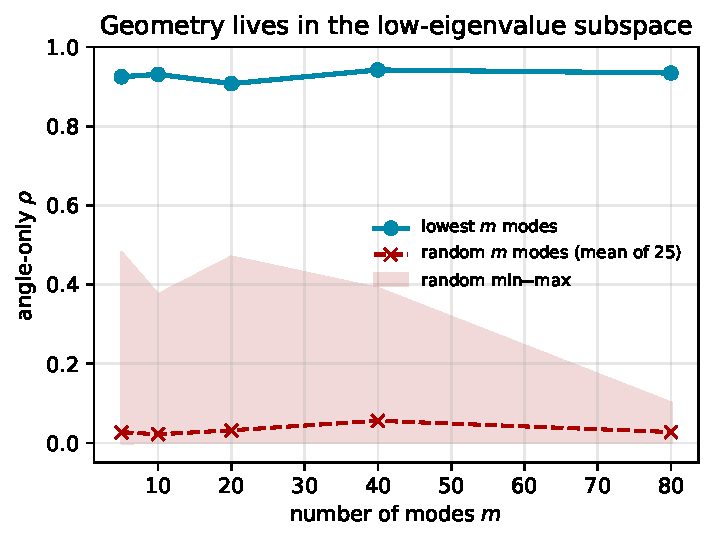
\includegraphics[width=\linewidth]{fig2_control.pdf}
\caption{Geometry lives in the low-eigenvalue subspace: lowest-$m$ modes preserve
geodesics; a random-mode basis of equal size does not. The random curve is the
mean over $25$ draws, the band its full min--max envelope---even the best-case
random draw stays far below the low-mode curve.}
\label{fig:control}
\end{minipage}
\end{figure}

\subsection{\texorpdfstring{Verifying Corollary~\ref{thm:radial} and
Conjecture~\ref{conj:angle}}{Verifying the degeneracy corollary and the angular
conjecture}}\label{sec:verify}
We check the two claims directly. The angle-$\rho$ is flat in graph size
while the full commute distance decays, and
the truncated radius tracks degree ($\rho(\lVert\Psi_i\rVert,1/\sqrt{k_i})=
0.79$--$0.87$ across $m=5$--$40$; radius-only $\rho\le0.08$). For the full
\emph{unnormalized} commute radius the degeneracy is exact,
Corollary~\ref{thm:radial} holding cleanly
at $d=3$ ($\rho(R,1/k_i+1/k_j)\to0.98$); $d=2$ is borderline (log corrections);
the quasi-1D case correctly shows no degeneracy, as the dimension gating
predicts. Conjecture~\ref{conj:angle}: in an $m$-sweep at $n=4000$, angle-$\rho$
is flat $\approx0.93$ across $m=5$--$80$ while the full embedding decays
$0.773\to0.437$.

\subsection{Which weighting carries the angle?}\label{sec:ablation}
The direction depends on the per-mode weight, so we ablate it on the torus
($d{=}2$) and a $3$-torus ($d{=}3$). Plain eigenmaps ($w_k{=}1$) give an angle
that \emph{collapses} with mode count---angle-$\rho$ falls from $0.554\pm0.013$ at
$m{=}10$ to $0.081\pm0.012$ at $m{=}20$ (five independent draws, $d{=}2$)---because
equal weighting lets high modes swamp the direction. The commute weight
$1/\sqrt{\lambda_k}$ is flat instead ($0.918\pm0.006\to0.896\pm0.006$), as is
diffusion $e^{-\lambda_k t}$; both suppress high modes,
which is what the geometry needs. The ``flat in $m$'' property is thus a property
of the weighting, not of angles in general---and it selects the commute (or
diffusion) weight, not the plain eigenmap. Proposition~\ref{prop:plain} now
supplies the continuum mechanism: plain angular distances concentrate at
$\sqrt2$ with only an oscillatory, geometry-blind correction, while the
commute correction is the (low-pass, Green-type) kernel that carries the
ranks. Degree correction, by contrast, is
\emph{invisible} to the angle: dividing or multiplying each row by $\sqrt{k_i}$
(the diffusion-map convention and its opposite) leaves angle-$\rho$ unchanged to
three digits ($0.889$ either way), because a per-node radial factor cancels under
row-normalization---a direct confirmation that the degree lives in the radius
(Corollary~\ref{thm:radial}), not the angle.

\section{Discussion and Conclusion}\label{sec:disc}
\textbf{The primary result is basis-level and substrate-agnostic.} The angular
coordinate of the low-Laplacian embedding preserves geodesics while the radial
coordinate is degree/density nuisance---von~Luxburg-degenerate for the full,
unnormalized commute radius at $d\ge3$ (Corollary~\ref{thm:radial}), and
empirically degree-tracking for the truncated, normalized radius actually in use
(\S\ref{sec:verify}). This gives Ng--Jordan--Weiss
row-normalization a geodesic justification complementary to the cluster-separation
theory of \cite{schiebinger2015}, and places it in the same scale-from-direction
decomposition that recurs in vector and KV-cache compression \cite{polarquant2025}
---the quotient, not the discard, being what recurs. The empirical reach of the
basis across substrate families, its role as a manifold diagnostic, the compression
scope boundary (angular quantization fails for attention keys, where scale is
signal, not nuisance---condition (A2) of Theorem~\ref{thm:transfer}), and a scoped
physical interpretation are developed in the companion Paper~I.b~\cite{paperIb}.

\paragraph{Open problems.} Proving Conjecture~\ref{conj:angle} (rank form, and the
bi-Lipschitz strengthening) is now reduced, at fixed $m$, to the chart hypotheses
(H1)--(H3) plus a distance-ratio condition for rank (Corollary~\ref{cor:global},
Proposition~\ref{prop:rank}); the open core is the \emph{scale-dependent} commute
uniformity---fixed-scale uniformity in $m$ is proven for the heat filter and
refuted for the commute filter (Theorem~\ref{thm:heat},
Proposition~\ref{prop:weyl})---and graph transfer at growing spectral windows
(section~\ref{app:uniform}). Beyond the flat torus, where
Corollary~\ref{cor:torus} settles them, (H1)--(H3) must be checked directly---the
obstruction being the normalized upper bound, not the differential lower bound,
which never collapses (Proposition~\ref{prop:sigmamin}). Also open: extending Corollary~\ref{thm:radial} to
the truncated, normalized radius used in practice; synthesizing clean manifolds
above $d\approx2$; a dimension-adaptive basis that tunes mode-count and diffusion
time against the fidelity decay; and whether the diagnostic transfers to learned
representations (a preliminary probe is in the repository).

\paragraph{Reproducibility.} The confirming experiments of this paper---the torus
core result and controls, the theorem verification, the weighting ablation, and the
truncation/normalization checks---are fully reproducible locally
(NumPy/SciPy/NetworkX, CPU), each script emitting the exact committed result JSON in
the accompanying repository, \url{https://github.com/ahb-sjsu/the-angular-observer}
(pre-registered as \texttt{PREREG\_RUNG3/4} with dated amendments). The extended
empirical program and its reproducibility tiers are documented in the companion
Paper~I.b~\cite{paperIb}.

\appendix
\section{Proof of Corollary~\ref{thm:radial}}\label{app:radial}

The diagonal statement $L^+_{ii}\to1/k_i$ does not follow from the pairwise
resistance limits alone:
$R(i,j)=L^+_{ii}+L^+_{jj}-2L^+_{ij}$ fixes only those combinations, so a
summation argument must control the error it accumulates. Two inputs are used,
both explicit in the corollary's statement: \textbf{(i)} the \emph{uniform
multiplicative} form of the
von~Luxburg--Radl--Hein degeneracy---for $d\ge3$ graphs in their model there is
a sequence $\eta_n\to0$ with
\[
R(i,j)=\Big(\frac1{k_i}+\frac1{k_j}\Big)\,(1+\eta_{ij}),\qquad
\sup_{i\ne j}\lvert\eta_{ij}\rvert\le\eta_n
\]
(this multiplicative-uniform form is not stated verbatim by \cite{vonluxburg2014}
(their Corollaries~8--9 and Propositions~29--30):
they prove an \emph{additive} deviation bound on the rescaled commute distance,
uniform over $i\ne j$, together with two-sided degree bounds; dividing the
additive bound by $1/k_i+1/k_j$ and using the degree bounds yields the displayed
$\eta_n$); and \textbf{(ii)} a bounded degree ratio,
$k_{\max}/k_{\min}\le K$ for all $n$ (their graph models satisfy this with high
probability). Write $S:=\sum_j 1/k_j$ and note $S/n\le1/k_{\min}\le K/k_i$ for
every $i$ by (ii).

\emph{Step 1 (row sums).} $L^+$ annihilates constants ($L\mathbf1=0$ and
$L^+$ shares the range of $L$ on $\mathbf1^\perp$), so $\sum_j L^+_{ij}=0$: the
gauge. Summing $R(i,j)$ over $j\ne i$ and using the gauge,
\[
\sum_{j\ne i}R(i,j)
=(n-1)L^+_{ii}+\big(\operatorname{tr}L^+-L^+_{ii}\big)
-2\sum_{j\ne i}L^+_{ij}
=n\,L^+_{ii}+\operatorname{tr}L^+,
\]
since $\sum_{j\ne i}L^+_{ij}=-L^+_{ii}$. By (i) the same sum equals
\[
\sum_{j\ne i}\Big(\frac1{k_i}+\frac1{k_j}\Big)(1+\eta_{ij})
=\frac{n-2}{k_i}+S+e_i,
\qquad
\lvert e_i\rvert\le\eta_n\Big(\frac{n}{k_i}+S\Big).
\]
Equating and dividing by $n$,
\begin{equation}
L^{+}_{ii}=\frac1{k_i}+C_n-\frac{2}{n k_i}+\frac{e_i}{n},
\qquad
C_n:=\frac{S-\operatorname{tr}L^+}{n}\ \text{ (independent of $i$)} .
\tag{A.1}
\end{equation}

\emph{Step 2 (trace identity kills $C_n$).} Summing (A.1) over $i$:
$\operatorname{tr}L^+=S+nC_n-\tfrac2nS+\tfrac1n\sum_i e_i$. Substituting
$nC_n=S-\operatorname{tr}L^+$ and solving,
\[
\operatorname{tr}L^+=S\Big(1-\frac1n\Big)+\frac{1}{2n}\sum_i e_i,
\qquad\text{hence}\qquad
C_n=\frac{S}{n^2}-\frac{1}{2n^2}\sum_i e_i .
\]
Since $\lvert\sum_i e_i\rvert\le\eta_n\sum_i(n/k_i+S)=2\eta_n nS$, we get
$\lvert C_n\rvert\le S/n^2+\eta_n S/n\le(1/n+\eta_n)\,K/k_i$ for every $i$,
using (ii).

\emph{Step 3 (conclusion).} Feeding the bounds on $C_n$ and $e_i/n$ back into
(A.1),
\[
\Big\lvert L^+_{ii}-\frac1{k_i}\Big\rvert
\ \le\ \frac{(1/n+\eta_n)K}{k_i}+\frac{2}{nk_i}
+\frac{\eta_n}{k_i}\big(1+K\big)
\ \le\ \frac{C(K)\,\big(\eta_n+1/n\big)}{k_i},
\]
so $k_iL^+_{ii}\to1$ uniformly over nodes, i.e.\
$L^+_{ii}=(1/k_i)(1+o(1))$ and $\lVert\Phi_i\rVert=\sqrt{L^+_{ii}}
=(1/\sqrt{k_i})(1+o(1))$. \hfill$\qed$

Without (ii) the conclusion weakens gracefully: the same computation gives
$L^+_{ii}=1/k_i+O\big((\eta_n+1/n)\,S/n\big)$, an \emph{additive} error at the
harmonic-mean-degree scale, so the degeneracy survives at the pairwise level
($R\approx1/k_i+1/k_j$, which is (i)) even when per-node relative control is lost.
The $j{=}i$ term ($R(i,i)=0$ while $1/k_i+1/k_j=2/k_i$) is excluded from the sums,
which is why the $(n-2)/k_i$ bookkeeping appears.


\section*{Supplementary materials}
An online supplement collects the longer proofs and the extended continuum theory:
the conditional transfer theorem (\S\ref{app:proof}); the truncation-uniformity
results, the uniform lower angular bound and exact upper divergence on flat tori,
the spectral-filter phase diagram, and the Green-kernel rank-limit theorem
(\S\ref{app:uniform}). Every statement in the main article is self-contained; each
supplementary proof is cross-referenced from the result it establishes.

\begin{thebibliography}{99}
\bibitem{paperIb} A.~H.~Bond. \emph{Keep the Angle, in Practice: A
Substrate-Agnostic Manifold Diagnostic and Its Failure Modes} (Paper~I.b).
Manuscript, 2026.
\bibitem{bates2014} J.~Bates. The embedding dimension of Laplacian
eigenfunction maps. \emph{Applied and Computational Harmonic Analysis},
37(3):516--530, 2014.
\bibitem{belkin2003} M.~Belkin and P.~Niyogi. Laplacian eigenmaps for
dimensionality reduction and data representation. \emph{Neural Computation},
15(6):1373--1396, 2003.
\bibitem{belkin2007} M.~Belkin and P.~Niyogi. Convergence of Laplacian
eigenmaps. In \emph{Advances in Neural Information Processing Systems 19}, 2007.
\bibitem{berard1994} P.~B\'erard, G.~Besson, and S.~Gallot. Embedding
Riemannian manifolds by their heat kernel. \emph{Geometric and Functional
Analysis (GAFA)}, 4(4):373--398, 1994.
\bibitem{calder2022} J.~Calder and N.~Garc\'ia Trillos. Improved spectral
convergence rates for graph Laplacians on $\varepsilon$-graphs and $k$-NN graphs.
\emph{Applied and Computational Harmonic Analysis}, 60:123--175, 2022.
\bibitem{calderlewicka2022} J.~Calder, N.~Garc\'ia Trillos, and
M.~Lewicka. Lipschitz regularity of graph Laplacians on random data clouds.
\emph{SIAM Journal on Mathematical Analysis}, 54(1):1169--1222, 2022.
\bibitem{chengmishne} X.~Cheng and G.~Mishne. Spectral embedding norm:
looking deep into the spectrum of the graph Laplacian. \emph{SIAM Journal on
Imaging Sciences}, 13(2):1015--1048, 2020.
\bibitem{coifman2006} R.~Coifman and S.~Lafon. Diffusion maps. \emph{Applied and
Computational Harmonic Analysis}, 21(1):5--30, 2006.
\bibitem{daniels1950} H.~E.~Daniels. Rank correlation and population
models. \emph{Journal of the Royal Statistical Society, Series B},
12(2):171--181, 1950.
\bibitem{garciatrillos2018} N.~Garc\'ia Trillos and D.~Slep\v{c}ev. A
variational approach to the consistency of spectral clustering. \emph{Applied
and Computational Harmonic Analysis}, 45(2):239--281, 2018.
\bibitem{gorard2020} J.~Gorard. Some relativistic and gravitational properties of
the Wolfram model. \emph{Complex Systems}, 29(2):107--192, 2020.
\bibitem{gromov1987} M.~Gromov. Hyperbolic groups. In \emph{Essays in Group
Theory}, MSRI Publications 8, pp.~75--263, Springer, 1987.
\bibitem{polarquant2025} I.~Han, P.~Kacham, A.~Karbasi, V.~Mirrokni, and
A.~Zandieh. PolarQuant: Quantizing KV caches with polar transformation.
\emph{arXiv preprint arXiv:2502.02617}, 2025.
\url{https://arxiv.org/abs/2502.02617}. Accessed July 2026.
\bibitem{jin2015score} J.~Jin. Fast community detection by SCORE.
\emph{The Annals of Statistics}, 43(1):57--89, 2015.
\bibitem{jones2010} P.~W.~Jones, M.~Maggioni, and R.~Schul. Universal local
parametrizations via heat kernels and eigenfunctions of the Laplacian.
\emph{Annales Academi\ae\ Scientiarum Fennic\ae\ Mathematica}, 35:131--174, 2010.
\bibitem{ng2002} A.~Ng, M.~Jordan, and Y.~Weiss. On spectral clustering:
analysis and an algorithm. \emph{Advances in Neural Information
Processing Systems 14 (NIPS)}, 2002.
\bibitem{nickel2017} M.~Nickel and D.~Kiela. Poincar\'e embeddings for learning
hierarchical representations. \emph{Advances in Neural Information
Processing Systems 30 (NIPS)}, 2017.
\bibitem{portegies2016} J.~W.~Portegies. Embeddings of Riemannian manifolds
with heat kernels and eigenfunctions. \emph{Communications on Pure and Applied
Mathematics}, 69(3):478--518, 2016.
\bibitem{qinrohe2013} T.~Qin and K.~Rohe. Regularized spectral clustering
under the degree-corrected stochastic blockmodel. \emph{Advances in Neural
Information Processing Systems 26 (NIPS)}, 2013.
\bibitem{rustamov2007} R.~M.~Rustamov. Laplace--Beltrami eigenfunctions for
deformation invariant shape representation. \emph{Proceedings of the Fifth
Eurographics Symposium on Geometry Processing (SGP)}, pp.~225--233, 2007.
\bibitem{sarkar2011} R.~Sarkar. Low-distortion delta-hyperbolic embedding in the
hyperbolic plane. \emph{Graph Drawing}, LNCS 7034, pp.~355--366, Springer,
2011.
\bibitem{schiebinger2015} G.~Schiebinger, M.~J.~Wainwright, and B.~Yu. The
geometry of kernelized spectral clustering. \emph{Annals of Statistics},
43(2):819--846, 2015.
\bibitem{sharma2012} A.~Sharma, R.~P.~Horaud, and D.~Mateus. 3D shape
registration using spectral graph embedding and probabilistic matching. In
O.~L\'ezoray and L.~Grady, editors, \emph{Image Processing and Analysis with
Graphs: Theory and Practice}, pp.~441--474. CRC Press, 2012.
\url{https://arxiv.org/abs/2106.11166}.
\bibitem{vonluxburg2008} U.~von~Luxburg, M.~Belkin, and O.~Bousquet.
Consistency of spectral clustering. \emph{Annals of Statistics},
36(2):555--586, 2008.
\bibitem{vonluxburg2014} U.~von~Luxburg, A.~Radl, and M.~Hein. Hitting and
commute times in large random neighborhood graphs. \emph{JMLR},
15:1751--1798, 2014.
\bibitem{wolfram2020} S.~Wolfram. Finally we may have a path to the fundamental
theory of physics\ldots and it's beautiful. Writings blog, April 2020.
\url{https://writings.stephenwolfram.com/2020/04/finally-we-may-have-a-path-to-the-fundamental-theory-of-physics-and-its-beautiful/}. Accessed July 2026.
\end{thebibliography}

\end{document}
